\documentclass[twoside]{book}

% Packages required by doxygen
\usepackage{fixltx2e}
\usepackage{calc}
\usepackage{doxygen}
\usepackage[export]{adjustbox} % also loads graphicx
\usepackage{graphicx}
\usepackage[utf8]{inputenc}
\usepackage{makeidx}
\usepackage{multicol}
\usepackage{multirow}
\PassOptionsToPackage{warn}{textcomp}
\usepackage{textcomp}
\usepackage[nointegrals]{wasysym}
\usepackage[table]{xcolor}

% Font selection
\usepackage[T1]{fontenc}
\usepackage[scaled=.90]{helvet}
\usepackage{courier}
\usepackage{amssymb}
\usepackage{sectsty}
\renewcommand{\familydefault}{\sfdefault}
\allsectionsfont{%
  \fontseries{bc}\selectfont%
  \color{darkgray}%
}
\renewcommand{\DoxyLabelFont}{%
  \fontseries{bc}\selectfont%
  \color{darkgray}%
}
\newcommand{\+}{\discretionary{\mbox{\scriptsize$\hookleftarrow$}}{}{}}

% Page & text layout
\usepackage{geometry}
\geometry{%
  a4paper,%
  top=2.5cm,%
  bottom=2.5cm,%
  left=2.5cm,%
  right=2.5cm%
}
\tolerance=750
\hfuzz=15pt
\hbadness=750
\setlength{\emergencystretch}{15pt}
\setlength{\parindent}{0cm}
\setlength{\parskip}{3ex plus 2ex minus 2ex}
\makeatletter
\renewcommand{\paragraph}{%
  \@startsection{paragraph}{4}{0ex}{-1.0ex}{1.0ex}{%
    \normalfont\normalsize\bfseries\SS@parafont%
  }%
}
\renewcommand{\subparagraph}{%
  \@startsection{subparagraph}{5}{0ex}{-1.0ex}{1.0ex}{%
    \normalfont\normalsize\bfseries\SS@subparafont%
  }%
}
\makeatother

% Headers & footers
\usepackage{fancyhdr}
\pagestyle{fancyplain}
\fancyhead[LE]{\fancyplain{}{\bfseries\thepage}}
\fancyhead[CE]{\fancyplain{}{}}
\fancyhead[RE]{\fancyplain{}{\bfseries\leftmark}}
\fancyhead[LO]{\fancyplain{}{\bfseries\rightmark}}
\fancyhead[CO]{\fancyplain{}{}}
\fancyhead[RO]{\fancyplain{}{\bfseries\thepage}}
\fancyfoot[LE]{\fancyplain{}{}}
\fancyfoot[CE]{\fancyplain{}{}}
\fancyfoot[RE]{\fancyplain{}{\bfseries\scriptsize Generated by Doxygen }}
\fancyfoot[LO]{\fancyplain{}{\bfseries\scriptsize Generated by Doxygen }}
\fancyfoot[CO]{\fancyplain{}{}}
\fancyfoot[RO]{\fancyplain{}{}}
\renewcommand{\footrulewidth}{0.4pt}
\renewcommand{\chaptermark}[1]{%
  \markboth{#1}{}%
}
\renewcommand{\sectionmark}[1]{%
  \markright{\thesection\ #1}%
}

% Indices & bibliography
\usepackage{natbib}
\usepackage[titles]{tocloft}
\setcounter{tocdepth}{3}
\setcounter{secnumdepth}{5}
\makeindex

% Hyperlinks (required, but should be loaded last)
\usepackage{ifpdf}
\ifpdf
  \usepackage[pdftex,pagebackref=true]{hyperref}
\else
  \usepackage[ps2pdf,pagebackref=true]{hyperref}
\fi
\hypersetup{%
  colorlinks=true,%
  linkcolor=blue,%
  citecolor=blue,%
  unicode%
}

% Custom commands
\newcommand{\clearemptydoublepage}{%
  \newpage{\pagestyle{empty}\cleardoublepage}%
}

\usepackage{caption}
\captionsetup{labelsep=space,justification=centering,font={bf},singlelinecheck=off,skip=4pt,position=top}

%===== C O N T E N T S =====

\begin{document}

% Titlepage & ToC
\hypersetup{pageanchor=false,
             bookmarksnumbered=true,
             pdfencoding=unicode
            }
\pagenumbering{alph}
\begin{titlepage}
\vspace*{7cm}
\begin{center}%
{\Large My Project }\\
\vspace*{1cm}
{\large Generated by Doxygen 1.8.13}\\
\end{center}
\end{titlepage}
\clearemptydoublepage
\pagenumbering{roman}
\tableofcontents
\clearemptydoublepage
\pagenumbering{arabic}
\hypersetup{pageanchor=true}

%--- Begin generated contents ---
\chapter{Hierarchical Index}
\section{Class Hierarchy}
This inheritance list is sorted roughly, but not completely, alphabetically\+:\begin{DoxyCompactList}
\item \contentsline{section}{IF}{\pageref{classIF}}{}
\begin{DoxyCompactList}
\item \contentsline{section}{L\+IF}{\pageref{classLIF}}{}
\end{DoxyCompactList}
\end{DoxyCompactList}

\chapter{Class Index}
\doxysection{Class List}
Here are the classes, structs, unions and interfaces with brief descriptions\+:\begin{DoxyCompactList}
\item\contentsline{section}{\mbox{\hyperlink{classCosineSignal}{Cosine\+Signal}} \\*Implements a cosine get\+\_\+value, i.\+e. alpha$\ast$cos(2$\ast$pi$\ast$f$\ast$t) }{\pageref{classCosineSignal}}{}
\item\contentsline{section}{\mbox{\hyperlink{classFiringRate}{Firing\+Rate}} \\*Abstract base class for firing rates. This is an abstract class that calculates the firing rate from given spike trains. One can add a spike train to a firing rate with the method add\+\_\+spike\+\_\+train, which will do the following\+: (i) it will increase the N\+\_\+neurons counter, which counts how many spike trains have been added overall and (ii) it will increase the number of spikes in the spikes histogram, which counts the spikes at a given time (these are of course determined by the time frame). One can calculate the firing rate by calling firing\+\_\+rate.\+calculate(). This of course depends on how one actually calculates the firing rate from given spike trains, which is implemented in the subclasses }{\pageref{classFiringRate}}{}
\item\contentsline{section}{\mbox{\hyperlink{classFiringRateBox}{Firing\+Rate\+Box}} \\*Implements a box firing rate. The box firing rate is calculated by counting the number of neuron that have spiked in a certain time interval (here given by the time step dt of the time frame) and dividing that number by N$\ast$dt, where N is the number of neurons overall }{\pageref{classFiringRateBox}}{}
\item\contentsline{section}{\mbox{\hyperlink{classFiringRateExp}{Firing\+Rate\+Exp}} \\*Implements an exponential firing rate. The exponential firing rate is calculated by convolving the spike train with a gaussian window function. See \cite{dayan05} }{\pageref{classFiringRateExp}}{}
\item\contentsline{section}{\mbox{\hyperlink{classFiringRateFactory}{Firing\+Rate\+Factory}} }{\pageref{classFiringRateFactory}}{}
\item\contentsline{section}{\mbox{\hyperlink{classFiringRateSimulation}{Firing\+Rate\+Simulation}} }{\pageref{classFiringRateSimulation}}{}
\item\contentsline{section}{\mbox{\hyperlink{classIF}{IF}} \\*An abstract base class for integrate-\/and-\/fire neurons }{\pageref{classIF}}{}
\item\contentsline{section}{\mbox{\hyperlink{classIFAC}{I\+F\+AC}} \\*An abstract base class for integrate-\/and-\/fire neurons with an adaptation current }{\pageref{classIFAC}}{}
\item\contentsline{section}{\mbox{\hyperlink{classLIF}{L\+IF}} \\*Implements a leaky integrate-\/and-\/fire (\mbox{\hyperlink{classLIF}{L\+IF}}) neuron }{\pageref{classLIF}}{}
\item\contentsline{section}{\mbox{\hyperlink{classLIFAC}{L\+I\+F\+AC}} \\*Implements a leaky integrate-\/and-\/fire (\mbox{\hyperlink{classLIFAC}{L\+I\+F\+AC}}) neuron }{\pageref{classLIFAC}}{}
\item\contentsline{section}{\mbox{\hyperlink{classNeuron}{Neuron}} }{\pageref{classNeuron}}{}
\item\contentsline{section}{\mbox{\hyperlink{classNeuronFactory}{Neuron\+Factory}} }{\pageref{classNeuronFactory}}{}
\item\contentsline{section}{\mbox{\hyperlink{classOptions}{Options}} \\*Implements a class that handles command line options }{\pageref{classOptions}}{}
\item\contentsline{section}{\mbox{\hyperlink{classPIF}{P\+IF}} \\*Implement a perfect integrate-\/and-\/fire (\mbox{\hyperlink{classPIF}{P\+IF}}) neuron }{\pageref{classPIF}}{}
\item\contentsline{section}{\mbox{\hyperlink{classPIFAC}{P\+I\+F\+AC}} \\*Implement a perfect integrate-\/and-\/fire (\mbox{\hyperlink{classPIFAC}{P\+I\+F\+AC}}) neuron }{\pageref{classPIFAC}}{}
\item\contentsline{section}{\mbox{\hyperlink{classSignal}{Signal}} \\*An abstract base class for signals }{\pageref{classSignal}}{}
\item\contentsline{section}{\mbox{\hyperlink{classSignalFactory}{Signal\+Factory}} \\*Implements the factory design pattern for \mbox{\hyperlink{classSignal}{Signal}} }{\pageref{classSignalFactory}}{}
\item\contentsline{section}{\mbox{\hyperlink{classSimulation}{Simulation}} }{\pageref{classSimulation}}{}
\item\contentsline{section}{\mbox{\hyperlink{classSpikeTrain}{Spike\+Train}} }{\pageref{classSpikeTrain}}{}
\item\contentsline{section}{\mbox{\hyperlink{classStepSignal}{Step\+Signal}} \\*Implement a step get\+\_\+value, i.\+e. alpha$\ast$\+Theta(t -\/ t\+\_\+0) }{\pageref{classStepSignal}}{}
\item\contentsline{section}{\mbox{\hyperlink{classTimeFrame}{Time\+Frame}} \\*A time frame class }{\pageref{classTimeFrame}}{}
\item\contentsline{section}{\mbox{\hyperlink{classTwoCosineSignal}{Two\+Cosine\+Signal}} \\*Implements a get\+\_\+value consisting of two cosine, i.\+e. alpha$\ast$cos(2$\ast$pi$\ast$f1$\ast$t) }{\pageref{classTwoCosineSignal}}{}
\item\contentsline{section}{\mbox{\hyperlink{classWhiteNoiseSignal}{White\+Noise\+Signal}} \\*Implements a band limited white gaussian noise get\+\_\+value }{\pageref{classWhiteNoiseSignal}}{}
\end{DoxyCompactList}

\chapter{Class Documentation}
\hypertarget{classAdaptation}{}\section{Adaptation Class Reference}
\label{classAdaptation}\index{Adaptation@{Adaptation}}


Implements an abstract base class for adaptation variable.  




{\ttfamily \#include $<$Adaptation.\+h$>$}

\subsection*{Public Member Functions}
\begin{DoxyCompactItemize}
\item 
virtual double \hyperlink{classAdaptation_a4c7f62690bb8639a307c0ed840890e30}{adapt} (double a, double t) const =0
\begin{DoxyCompactList}\small\item\em Returns the \char`\"{}right side\char`\"{} of the equation for the adaptation variable, i.\+e. f(a,t) = da/dt. \end{DoxyCompactList}\item 
virtual double \hyperlink{classAdaptation_a146da63f54c22a3c08c2c5ce26f11f66}{reset\+\_\+rule} (double a) const =0
\begin{DoxyCompactList}\small\item\em Reset rule for the adaptation variable. \end{DoxyCompactList}\end{DoxyCompactItemize}


\subsection{Detailed Description}
Implements an abstract base class for adaptation variable. 

\subsection{Member Function Documentation}
\mbox{\Hypertarget{classAdaptation_a4c7f62690bb8639a307c0ed840890e30}\label{classAdaptation_a4c7f62690bb8639a307c0ed840890e30}} 
\index{Adaptation@{Adaptation}!adapt@{adapt}}
\index{adapt@{adapt}!Adaptation@{Adaptation}}
\subsubsection{\texorpdfstring{adapt()}{adapt()}}
{\footnotesize\ttfamily virtual double Adaptation\+::adapt (\begin{DoxyParamCaption}\item[{double}]{a,  }\item[{double}]{t }\end{DoxyParamCaption}) const\hspace{0.3cm}{\ttfamily [pure virtual]}}



Returns the \char`\"{}right side\char`\"{} of the equation for the adaptation variable, i.\+e. f(a,t) = da/dt. 


\begin{DoxyParams}{Parameters}
{\em a} & \hyperlink{classAdaptation}{Adaptation} variable. \\
\hline
{\em t} & Time \\
\hline
\end{DoxyParams}
\begin{DoxyReturn}{Returns}
The time derivative da/dt 
\end{DoxyReturn}


Implemented in \hyperlink{classExpAdaptation_aef5119a0f09698f1526938f04654e3f4}{Exp\+Adaptation}.

\mbox{\Hypertarget{classAdaptation_a146da63f54c22a3c08c2c5ce26f11f66}\label{classAdaptation_a146da63f54c22a3c08c2c5ce26f11f66}} 
\index{Adaptation@{Adaptation}!reset\+\_\+rule@{reset\+\_\+rule}}
\index{reset\+\_\+rule@{reset\+\_\+rule}!Adaptation@{Adaptation}}
\subsubsection{\texorpdfstring{reset\+\_\+rule()}{reset\_rule()}}
{\footnotesize\ttfamily virtual double Adaptation\+::reset\+\_\+rule (\begin{DoxyParamCaption}\item[{double}]{a }\end{DoxyParamCaption}) const\hspace{0.3cm}{\ttfamily [pure virtual]}}



Reset rule for the adaptation variable. 


\begin{DoxyParams}{Parameters}
{\em a} & \hyperlink{classAdaptation}{Adaptation} variable \\
\hline
\end{DoxyParams}
\begin{DoxyReturn}{Returns}
The reset adaptation variable 
\end{DoxyReturn}


Implemented in \hyperlink{classExpAdaptation_ac194bba0fd15aea6a68b8964a21fff2d}{Exp\+Adaptation}.



The documentation for this class was generated from the following file\+:\begin{DoxyCompactItemize}
\item 
/users/stud/egerlanc/\+Repos/\+Master/\+Spike/src/\+Adaptation/Adaptation.\+h\end{DoxyCompactItemize}

\hypertarget{classCosineSignal}{}\doxysection{Cosine\+Signal Class Reference}
\label{classCosineSignal}\index{CosineSignal@{CosineSignal}}


Implements a cosine get\+\_\+value, i.\+e. alpha$\ast$cos(2$\ast$pi$\ast$f$\ast$t)  




{\ttfamily \#include $<$Cosine\+Signal.\+h$>$}

\doxysubsection*{Public Member Functions}
\begin{DoxyCompactItemize}
\item 
\mbox{\hyperlink{classCosineSignal_ab4df140ccdbbf7eb1138647eb53a5100}{Cosine\+Signal}} (double alpha, double f, const \mbox{\hyperlink{classTimeFrame}{Time\+Frame}} \&\mbox{\hyperlink{classSignal_a47f018d11758cab322d1187b9392c1f9}{time\+\_\+frame}})
\begin{DoxyCompactList}\small\item\em Construct \mbox{\hyperlink{classCosineSignal}{Cosine\+Signal}} from parameters. \end{DoxyCompactList}\item 
\mbox{\hyperlink{classCosineSignal_ad69d9fa507d81bbb3db79bc1d3e4fc34}{Cosine\+Signal}} (const std\+::string \&input\+\_\+file, const \mbox{\hyperlink{classTimeFrame}{Time\+Frame}} \&\mbox{\hyperlink{classSignal_a47f018d11758cab322d1187b9392c1f9}{time\+\_\+frame}})
\begin{DoxyCompactList}\small\item\em Construct \mbox{\hyperlink{classCosineSignal}{Cosine\+Signal}} from input file. \end{DoxyCompactList}\item 
\mbox{\Hypertarget{classCosineSignal_a117f1ddb1b7cbdacbf179891ff440229}\label{classCosineSignal_a117f1ddb1b7cbdacbf179891ff440229}} 
void \mbox{\hyperlink{classCosineSignal_a117f1ddb1b7cbdacbf179891ff440229}{calculate\+\_\+signal}} ()
\begin{DoxyCompactList}\small\item\em Calculates the cosine get\+\_\+value. \end{DoxyCompactList}\item 
double \mbox{\hyperlink{classCosineSignal_a541f39de155f6a92162882ce102480bd}{signal}} (double t) const
\begin{DoxyCompactList}\small\item\em Returns get\+\_\+value, i.\+e. alpha$\ast$cos(2$\ast$pi$\ast$f$\ast$t) \end{DoxyCompactList}\item 
double \mbox{\hyperlink{classCosineSignal_ae4d286b605aa34aca31619f121fe0b41}{get\+\_\+f}} () const
\begin{DoxyCompactList}\small\item\em Getter function for the frequency. \end{DoxyCompactList}\item 
\mbox{\Hypertarget{classCosineSignal_aa67c5fac7f32cac4f2f21748dcfb7a32}\label{classCosineSignal_aa67c5fac7f32cac4f2f21748dcfb7a32}} 
void {\bfseries print\+\_\+info} (std\+::ofstream \&file) override
\end{DoxyCompactItemize}
\doxysubsection*{Additional Inherited Members}


\doxysubsection{Detailed Description}
Implements a cosine get\+\_\+value, i.\+e. alpha$\ast$cos(2$\ast$pi$\ast$f$\ast$t) 

\doxysubsection{Constructor \& Destructor Documentation}
\mbox{\Hypertarget{classCosineSignal_ab4df140ccdbbf7eb1138647eb53a5100}\label{classCosineSignal_ab4df140ccdbbf7eb1138647eb53a5100}} 
\index{CosineSignal@{CosineSignal}!CosineSignal@{CosineSignal}}
\index{CosineSignal@{CosineSignal}!CosineSignal@{CosineSignal}}
\doxysubsubsection{\texorpdfstring{CosineSignal()}{CosineSignal()}\hspace{0.1cm}{\footnotesize\ttfamily [1/2]}}
{\footnotesize\ttfamily Cosine\+Signal\+::\+Cosine\+Signal (\begin{DoxyParamCaption}\item[{double}]{alpha,  }\item[{double}]{f,  }\item[{const \mbox{\hyperlink{classTimeFrame}{Time\+Frame}} \&}]{time\+\_\+frame }\end{DoxyParamCaption})}



Construct \mbox{\hyperlink{classCosineSignal}{Cosine\+Signal}} from parameters. 


\begin{DoxyParams}{Parameters}
{\em alpha} & Amplitude \\
\hline
{\em f} & Frequency \\
\hline
{\em time\+\_\+frame} & \mbox{\hyperlink{classTimeFrame}{Time\+Frame}} \\
\hline
\end{DoxyParams}
\mbox{\Hypertarget{classCosineSignal_ad69d9fa507d81bbb3db79bc1d3e4fc34}\label{classCosineSignal_ad69d9fa507d81bbb3db79bc1d3e4fc34}} 
\index{CosineSignal@{CosineSignal}!CosineSignal@{CosineSignal}}
\index{CosineSignal@{CosineSignal}!CosineSignal@{CosineSignal}}
\doxysubsubsection{\texorpdfstring{CosineSignal()}{CosineSignal()}\hspace{0.1cm}{\footnotesize\ttfamily [2/2]}}
{\footnotesize\ttfamily Cosine\+Signal\+::\+Cosine\+Signal (\begin{DoxyParamCaption}\item[{const std\+::string \&}]{input\+\_\+file,  }\item[{const \mbox{\hyperlink{classTimeFrame}{Time\+Frame}} \&}]{time\+\_\+frame }\end{DoxyParamCaption})}



Construct \mbox{\hyperlink{classCosineSignal}{Cosine\+Signal}} from input file. 


\begin{DoxyParams}{Parameters}
{\em input\+\_\+file} & Input file in .json format \\
\hline
{\em time\+\_\+frame} & \mbox{\hyperlink{classTimeFrame}{Time\+Frame}} \\
\hline
\end{DoxyParams}


\doxysubsection{Member Function Documentation}
\mbox{\Hypertarget{classCosineSignal_ae4d286b605aa34aca31619f121fe0b41}\label{classCosineSignal_ae4d286b605aa34aca31619f121fe0b41}} 
\index{CosineSignal@{CosineSignal}!get\_f@{get\_f}}
\index{get\_f@{get\_f}!CosineSignal@{CosineSignal}}
\doxysubsubsection{\texorpdfstring{get\_f()}{get\_f()}}
{\footnotesize\ttfamily double Cosine\+Signal\+::get\+\_\+f (\begin{DoxyParamCaption}{ }\end{DoxyParamCaption}) const\hspace{0.3cm}{\ttfamily [inline]}}



Getter function for the frequency. 

\begin{DoxyReturn}{Returns}
The frequency of the get\+\_\+value f 
\end{DoxyReturn}
\mbox{\Hypertarget{classCosineSignal_a541f39de155f6a92162882ce102480bd}\label{classCosineSignal_a541f39de155f6a92162882ce102480bd}} 
\index{CosineSignal@{CosineSignal}!signal@{signal}}
\index{signal@{signal}!CosineSignal@{CosineSignal}}
\doxysubsubsection{\texorpdfstring{signal()}{signal()}}
{\footnotesize\ttfamily double Cosine\+Signal\+::signal (\begin{DoxyParamCaption}\item[{double}]{t }\end{DoxyParamCaption}) const}



Returns get\+\_\+value, i.\+e. alpha$\ast$cos(2$\ast$pi$\ast$f$\ast$t) 


\begin{DoxyParams}{Parameters}
{\em t} & Time \\
\hline
\end{DoxyParams}
\begin{DoxyReturn}{Returns}
\mbox{\hyperlink{classSignal}{Signal}}, i.\+e. alpha$\ast$cos(2$\ast$pi$\ast$f$\ast$t) 
\end{DoxyReturn}


The documentation for this class was generated from the following files\+:\begin{DoxyCompactItemize}
\item 
/home/cheg/\+Repos/\+Master/\+Spike/src/\+Signal/Cosine\+Signal.\+h\item 
/home/cheg/\+Repos/\+Master/\+Spike/src/\+Signal/Cosine\+Signal.\+cpp\end{DoxyCompactItemize}

\hypertarget{classExpAdaptation}{}\section{Exp\+Adaptation Class Reference}
\label{classExpAdaptation}\index{Exp\+Adaptation@{Exp\+Adaptation}}


Implements the exponential adaptation, i.\+e. where adaptation variable follows the equation tau\+\_\+a da/dt = -\/a, with the reset rule a -\/$>$ a + Delta.  




{\ttfamily \#include $<$Exp\+Adaptation.\+h$>$}

\subsection*{Public Member Functions}
\begin{DoxyCompactItemize}
\item 
\hyperlink{classExpAdaptation_a7cf74c9283d78b47b2ee49cf9bf4b3c3}{Exp\+Adaptation} (double Delta, double tau\+\_\+a)
\begin{DoxyCompactList}\small\item\em Constructs \hyperlink{classExpAdaptation}{Exp\+Adaptation} from parameters. \end{DoxyCompactList}\item 
\hyperlink{classExpAdaptation_a451a3bb8244dcd086d05c06a54865568}{Exp\+Adaptation} (const std\+::string \&input\+\_\+file)
\begin{DoxyCompactList}\small\item\em Constructs \hyperlink{classExpAdaptation}{Exp\+Adaptation} from input\+\_\+file. \end{DoxyCompactList}\item 
double \hyperlink{classExpAdaptation_aef5119a0f09698f1526938f04654e3f4}{adapt} (double a, double t) const
\begin{DoxyCompactList}\small\item\em Returns da/dt = -\/1/tau\+\_\+a $\ast$ a. \end{DoxyCompactList}\item 
double \hyperlink{classExpAdaptation_ac194bba0fd15aea6a68b8964a21fff2d}{reset\+\_\+rule} (double a) const
\begin{DoxyCompactList}\small\item\em Reset rule for adaptation variable. \end{DoxyCompactList}\item 
double \hyperlink{classExpAdaptation_ab99255b3adfe6fc0f2fcf2992f520565}{get\+\_\+\+Delta} () const
\begin{DoxyCompactList}\small\item\em Getter method for Delta. \end{DoxyCompactList}\item 
double \hyperlink{classExpAdaptation_a2fab2ad7a21e78b6984116132aed2836}{get\+\_\+tau\+\_\+a} () const
\begin{DoxyCompactList}\small\item\em Getter method for tau\+\_\+a. \end{DoxyCompactList}\item 
void \hyperlink{classExpAdaptation_aec93194aa8a695cbb26c47c40469a153}{set\+\_\+\+Delta} (double Delta)
\begin{DoxyCompactList}\small\item\em Setter method for Delta. \end{DoxyCompactList}\item 
void \hyperlink{classExpAdaptation_a9093324d5aff70f75b82f302f698d468}{set\+\_\+tau\+\_\+a} (double tau\+\_\+a)
\begin{DoxyCompactList}\small\item\em Setter method for tau\+\_\+a. \end{DoxyCompactList}\end{DoxyCompactItemize}


\subsection{Detailed Description}
Implements the exponential adaptation, i.\+e. where adaptation variable follows the equation tau\+\_\+a da/dt = -\/a, with the reset rule a -\/$>$ a + Delta. 

\subsection{Constructor \& Destructor Documentation}
\mbox{\Hypertarget{classExpAdaptation_a7cf74c9283d78b47b2ee49cf9bf4b3c3}\label{classExpAdaptation_a7cf74c9283d78b47b2ee49cf9bf4b3c3}} 
\index{Exp\+Adaptation@{Exp\+Adaptation}!Exp\+Adaptation@{Exp\+Adaptation}}
\index{Exp\+Adaptation@{Exp\+Adaptation}!Exp\+Adaptation@{Exp\+Adaptation}}
\subsubsection{\texorpdfstring{Exp\+Adaptation()}{ExpAdaptation()}\hspace{0.1cm}{\footnotesize\ttfamily [1/2]}}
{\footnotesize\ttfamily Exp\+Adaptation\+::\+Exp\+Adaptation (\begin{DoxyParamCaption}\item[{double}]{Delta,  }\item[{double}]{tau\+\_\+a }\end{DoxyParamCaption})}



Constructs \hyperlink{classExpAdaptation}{Exp\+Adaptation} from parameters. 


\begin{DoxyParams}{Parameters}
{\em Delta} & Size of the kick \\
\hline
{\em tau\+\_\+a} & \hyperlink{classAdaptation}{Adaptation} time scale \\
\hline
\end{DoxyParams}
\mbox{\Hypertarget{classExpAdaptation_a451a3bb8244dcd086d05c06a54865568}\label{classExpAdaptation_a451a3bb8244dcd086d05c06a54865568}} 
\index{Exp\+Adaptation@{Exp\+Adaptation}!Exp\+Adaptation@{Exp\+Adaptation}}
\index{Exp\+Adaptation@{Exp\+Adaptation}!Exp\+Adaptation@{Exp\+Adaptation}}
\subsubsection{\texorpdfstring{Exp\+Adaptation()}{ExpAdaptation()}\hspace{0.1cm}{\footnotesize\ttfamily [2/2]}}
{\footnotesize\ttfamily Exp\+Adaptation\+::\+Exp\+Adaptation (\begin{DoxyParamCaption}\item[{const std\+::string \&}]{input\+\_\+file }\end{DoxyParamCaption})}



Constructs \hyperlink{classExpAdaptation}{Exp\+Adaptation} from input\+\_\+file. 


\begin{DoxyParams}{Parameters}
{\em input\+\_\+file} & Input file in .json format. \\
\hline
\end{DoxyParams}


\subsection{Member Function Documentation}
\mbox{\Hypertarget{classExpAdaptation_aef5119a0f09698f1526938f04654e3f4}\label{classExpAdaptation_aef5119a0f09698f1526938f04654e3f4}} 
\index{Exp\+Adaptation@{Exp\+Adaptation}!adapt@{adapt}}
\index{adapt@{adapt}!Exp\+Adaptation@{Exp\+Adaptation}}
\subsubsection{\texorpdfstring{adapt()}{adapt()}}
{\footnotesize\ttfamily double Exp\+Adaptation\+::adapt (\begin{DoxyParamCaption}\item[{double}]{a,  }\item[{double}]{t }\end{DoxyParamCaption}) const\hspace{0.3cm}{\ttfamily [virtual]}}



Returns da/dt = -\/1/tau\+\_\+a $\ast$ a. 


\begin{DoxyParams}{Parameters}
{\em a} & \hyperlink{classAdaptation}{Adaptation} current \\
\hline
{\em t} & time \\
\hline
\end{DoxyParams}
\begin{DoxyReturn}{Returns}
Returns da/dt = -\/1/tau\+\_\+a $\ast$ a 
\end{DoxyReturn}


Implements \hyperlink{classAdaptation_a4c7f62690bb8639a307c0ed840890e30}{Adaptation}.

\mbox{\Hypertarget{classExpAdaptation_ab99255b3adfe6fc0f2fcf2992f520565}\label{classExpAdaptation_ab99255b3adfe6fc0f2fcf2992f520565}} 
\index{Exp\+Adaptation@{Exp\+Adaptation}!get\+\_\+\+Delta@{get\+\_\+\+Delta}}
\index{get\+\_\+\+Delta@{get\+\_\+\+Delta}!Exp\+Adaptation@{Exp\+Adaptation}}
\subsubsection{\texorpdfstring{get\+\_\+\+Delta()}{get\_Delta()}}
{\footnotesize\ttfamily double Exp\+Adaptation\+::get\+\_\+\+Delta (\begin{DoxyParamCaption}{ }\end{DoxyParamCaption}) const\hspace{0.3cm}{\ttfamily [inline]}}



Getter method for Delta. 

\begin{DoxyReturn}{Returns}
Kick size Delta 
\end{DoxyReturn}
\mbox{\Hypertarget{classExpAdaptation_a2fab2ad7a21e78b6984116132aed2836}\label{classExpAdaptation_a2fab2ad7a21e78b6984116132aed2836}} 
\index{Exp\+Adaptation@{Exp\+Adaptation}!get\+\_\+tau\+\_\+a@{get\+\_\+tau\+\_\+a}}
\index{get\+\_\+tau\+\_\+a@{get\+\_\+tau\+\_\+a}!Exp\+Adaptation@{Exp\+Adaptation}}
\subsubsection{\texorpdfstring{get\+\_\+tau\+\_\+a()}{get\_tau\_a()}}
{\footnotesize\ttfamily double Exp\+Adaptation\+::get\+\_\+tau\+\_\+a (\begin{DoxyParamCaption}{ }\end{DoxyParamCaption}) const\hspace{0.3cm}{\ttfamily [inline]}}



Getter method for tau\+\_\+a. 

\begin{DoxyReturn}{Returns}
\hyperlink{classAdaptation}{Adaptation} time scale tau\+\_\+a 
\end{DoxyReturn}
\mbox{\Hypertarget{classExpAdaptation_ac194bba0fd15aea6a68b8964a21fff2d}\label{classExpAdaptation_ac194bba0fd15aea6a68b8964a21fff2d}} 
\index{Exp\+Adaptation@{Exp\+Adaptation}!reset\+\_\+rule@{reset\+\_\+rule}}
\index{reset\+\_\+rule@{reset\+\_\+rule}!Exp\+Adaptation@{Exp\+Adaptation}}
\subsubsection{\texorpdfstring{reset\+\_\+rule()}{reset\_rule()}}
{\footnotesize\ttfamily double Exp\+Adaptation\+::reset\+\_\+rule (\begin{DoxyParamCaption}\item[{double}]{a }\end{DoxyParamCaption}) const\hspace{0.3cm}{\ttfamily [virtual]}}



Reset rule for adaptation variable. 


\begin{DoxyParams}{Parameters}
{\em a} & \hyperlink{classAdaptation}{Adaptation} variable \\
\hline
\end{DoxyParams}
\begin{DoxyReturn}{Returns}
Returns a -\/$>$ a + Delta 
\end{DoxyReturn}


Implements \hyperlink{classAdaptation_a146da63f54c22a3c08c2c5ce26f11f66}{Adaptation}.

\mbox{\Hypertarget{classExpAdaptation_aec93194aa8a695cbb26c47c40469a153}\label{classExpAdaptation_aec93194aa8a695cbb26c47c40469a153}} 
\index{Exp\+Adaptation@{Exp\+Adaptation}!set\+\_\+\+Delta@{set\+\_\+\+Delta}}
\index{set\+\_\+\+Delta@{set\+\_\+\+Delta}!Exp\+Adaptation@{Exp\+Adaptation}}
\subsubsection{\texorpdfstring{set\+\_\+\+Delta()}{set\_Delta()}}
{\footnotesize\ttfamily void Exp\+Adaptation\+::set\+\_\+\+Delta (\begin{DoxyParamCaption}\item[{double}]{Delta }\end{DoxyParamCaption})\hspace{0.3cm}{\ttfamily [inline]}}



Setter method for Delta. 


\begin{DoxyParams}{Parameters}
{\em Delta} & New kick size \\
\hline
\end{DoxyParams}
\mbox{\Hypertarget{classExpAdaptation_a9093324d5aff70f75b82f302f698d468}\label{classExpAdaptation_a9093324d5aff70f75b82f302f698d468}} 
\index{Exp\+Adaptation@{Exp\+Adaptation}!set\+\_\+tau\+\_\+a@{set\+\_\+tau\+\_\+a}}
\index{set\+\_\+tau\+\_\+a@{set\+\_\+tau\+\_\+a}!Exp\+Adaptation@{Exp\+Adaptation}}
\subsubsection{\texorpdfstring{set\+\_\+tau\+\_\+a()}{set\_tau\_a()}}
{\footnotesize\ttfamily void Exp\+Adaptation\+::set\+\_\+tau\+\_\+a (\begin{DoxyParamCaption}\item[{double}]{tau\+\_\+a }\end{DoxyParamCaption})\hspace{0.3cm}{\ttfamily [inline]}}



Setter method for tau\+\_\+a. 


\begin{DoxyParams}{Parameters}
{\em tau\+\_\+a} & New adaptation time scale \\
\hline
\end{DoxyParams}


The documentation for this class was generated from the following files\+:\begin{DoxyCompactItemize}
\item 
/users/stud/egerlanc/\+Repos/\+Master/\+Spike/src/\+Adaptation/Exp\+Adaptation.\+h\item 
/users/stud/egerlanc/\+Repos/\+Master/\+Spike/src/\+Adaptation/Exp\+Adaptation.\+cpp\end{DoxyCompactItemize}

\hypertarget{classIF}{}\section{IF Class Reference}
\label{classIF}\index{IF@{IF}}


{\ttfamily \#include $<$models.\+h$>$}



Inheritance diagram for IF\+:\nopagebreak
\begin{figure}[H]
\begin{center}
\leavevmode
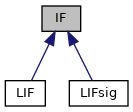
\includegraphics[width=111pt]{classIF__inherit__graph}
\end{center}
\end{figure}
\subsection*{Public Member Functions}
\begin{DoxyCompactItemize}
\item 
virtual double \hyperlink{classIF_a9bbd53df68cb9028bf87cf5273253e91}{drift} (double v, double t)
\item 
\mbox{\Hypertarget{classIF_a45c14ff90b19a93769c2c30741cd482d}\label{classIF_a45c14ff90b19a93769c2c30741cd482d}} 
virtual double {\bfseries diffusion} (double v, double t)
\end{DoxyCompactItemize}
\subsection*{Public Attributes}
\begin{DoxyCompactItemize}
\item 
int \hyperlink{classIF_aa81bddacf949214f2265214d7174f4c2}{N}
\item 
\mbox{\Hypertarget{classIF_ab9ff14c2b3690db446567d26cdf21540}\label{classIF_ab9ff14c2b3690db446567d26cdf21540}} 
double {\bfseries t\+\_\+0}
\item 
\mbox{\Hypertarget{classIF_a2c512964adfc0421306b655ba3c85d3d}\label{classIF_a2c512964adfc0421306b655ba3c85d3d}} 
double {\bfseries t\+\_\+end}
\item 
\mbox{\Hypertarget{classIF_a9f690c993d7b7cd0095e26607503db72}\label{classIF_a9f690c993d7b7cd0095e26607503db72}} 
double {\bfseries mu}
\item 
\mbox{\Hypertarget{classIF_a7e0fdbf32975dba0acf8096524885639}\label{classIF_a7e0fdbf32975dba0acf8096524885639}} 
double {\bfseries D}
\end{DoxyCompactItemize}


\subsection{Detailed Description}
Defines the integrate and fire (\hyperlink{classIF}{IF}) neuron, defaults to perfect \hyperlink{classIF}{IF} 

\subsection{Member Function Documentation}
\mbox{\Hypertarget{classIF_a9bbd53df68cb9028bf87cf5273253e91}\label{classIF_a9bbd53df68cb9028bf87cf5273253e91}} 
\index{IF@{IF}!drift@{drift}}
\index{drift@{drift}!IF@{IF}}
\subsubsection{\texorpdfstring{drift()}{drift()}}
{\footnotesize\ttfamily virtual double I\+F\+::drift (\begin{DoxyParamCaption}\item[{double}]{v,  }\item[{double}]{t }\end{DoxyParamCaption})\hspace{0.3cm}{\ttfamily [inline]}, {\ttfamily [virtual]}}

drift and diffusion functions, can be overwritten by subclasses 

Reimplemented in \hyperlink{classLIF_aea677a0cf3f943edb7a957479e18d6dc}{L\+IF}.



\subsection{Member Data Documentation}
\mbox{\Hypertarget{classIF_aa81bddacf949214f2265214d7174f4c2}\label{classIF_aa81bddacf949214f2265214d7174f4c2}} 
\index{IF@{IF}!N@{N}}
\index{N@{N}!IF@{IF}}
\subsubsection{\texorpdfstring{N}{N}}
{\footnotesize\ttfamily int I\+F\+::N}

Simulation parameters 
\begin{DoxyParams}{Parameters}
{\em N} & Number of times steps \\
\hline
{\em t\+\_\+0} & Starting time \\
\hline
{\em t\+\_\+end} & End time \\
\hline
{\em mu} & \\
\hline
{\em D} & Diffusion coefficient \\
\hline
\end{DoxyParams}


The documentation for this class was generated from the following file\+:\begin{DoxyCompactItemize}
\item 
/home/cheg/\+Repos/\+Master/\+Spike/src/models.\+h\end{DoxyCompactItemize}

\hypertarget{classLIF}{}\section{L\+IF Class Reference}
\label{classLIF}\index{L\+IF@{L\+IF}}


{\ttfamily \#include $<$models.\+h$>$}



Inheritance diagram for L\+IF\+:\nopagebreak
\begin{figure}[H]
\begin{center}
\leavevmode
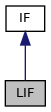
\includegraphics[width=111pt]{classLIF__inherit__graph}
\end{center}
\end{figure}


Collaboration diagram for L\+IF\+:\nopagebreak
\begin{figure}[H]
\begin{center}
\leavevmode
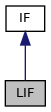
\includegraphics[width=111pt]{classLIF__coll__graph}
\end{center}
\end{figure}
\subsection*{Public Member Functions}
\begin{DoxyCompactItemize}
\item 
double \hyperlink{classLIF_aea677a0cf3f943edb7a957479e18d6dc}{drift} (double v, double t)
\end{DoxyCompactItemize}
\subsection*{Additional Inherited Members}


\subsection{Detailed Description}
Defines leaky integrate and fire neuron, inherits everything from \hyperlink{classIF}{IF} 

\subsection{Member Function Documentation}
\mbox{\Hypertarget{classLIF_aea677a0cf3f943edb7a957479e18d6dc}\label{classLIF_aea677a0cf3f943edb7a957479e18d6dc}} 
\index{L\+IF@{L\+IF}!drift@{drift}}
\index{drift@{drift}!L\+IF@{L\+IF}}
\subsubsection{\texorpdfstring{drift()}{drift()}}
{\footnotesize\ttfamily double L\+I\+F\+::drift (\begin{DoxyParamCaption}\item[{double}]{v,  }\item[{double}]{t }\end{DoxyParamCaption})\hspace{0.3cm}{\ttfamily [inline]}, {\ttfamily [virtual]}}

change the drift 

Reimplemented from \hyperlink{classIF_a9bbd53df68cb9028bf87cf5273253e91}{IF}.



The documentation for this class was generated from the following file\+:\begin{DoxyCompactItemize}
\item 
/home/cheg/\+Repos/\+Master/\+Spike/src/\+Models/models.\+h\end{DoxyCompactItemize}

\hypertarget{classOptions}{}\doxysection{Options Class Reference}
\label{classOptions}\index{Options@{Options}}


Implements a class that handles command line options.  




{\ttfamily \#include $<$Options.\+h$>$}

\doxysubsection*{Public Member Functions}
\begin{DoxyCompactItemize}
\item 
\mbox{\hyperlink{classOptions_aa1e7b11260c48cbc4d4c52266c74abf2}{Options}} (std\+::string input\+\_\+file)
\begin{DoxyCompactList}\small\item\em Construct \mbox{\hyperlink{classOptions}{Options}} from input file. \end{DoxyCompactList}\item 
\mbox{\hyperlink{classOptions_ab3a4819d972a234777923d85122bcf37}{Options}} (int argc, char $\ast$argv\mbox{[}$\,$\mbox{]})
\begin{DoxyCompactList}\small\item\em Construct \mbox{\hyperlink{classOptions}{Options}} from command line arguments. \end{DoxyCompactList}\item 
void \mbox{\hyperlink{classOptions_ab8ca4093f5561de9be0405380044c2ea}{check}} ()
\begin{DoxyCompactList}\small\item\em Checks the given input file. \end{DoxyCompactList}\item 
std\+::string \mbox{\hyperlink{classOptions_a76a7d420bed6ba601f1a222e8b81c9f9}{get\+\_\+input\+\_\+file}} () const
\begin{DoxyCompactList}\small\item\em Getter method for input file. \end{DoxyCompactList}\item 
std\+::string \mbox{\hyperlink{classOptions_a568c9513fefaf32d3834137506aacbcb}{get\+\_\+output\+\_\+file}} () const
\begin{DoxyCompactList}\small\item\em Getter method for output file. \end{DoxyCompactList}\end{DoxyCompactItemize}


\doxysubsection{Detailed Description}
Implements a class that handles command line options. 

\doxysubsection{Constructor \& Destructor Documentation}
\mbox{\Hypertarget{classOptions_aa1e7b11260c48cbc4d4c52266c74abf2}\label{classOptions_aa1e7b11260c48cbc4d4c52266c74abf2}} 
\index{Options@{Options}!Options@{Options}}
\index{Options@{Options}!Options@{Options}}
\doxysubsubsection{\texorpdfstring{Options()}{Options()}\hspace{0.1cm}{\footnotesize\ttfamily [1/2]}}
{\footnotesize\ttfamily Options\+::\+Options (\begin{DoxyParamCaption}\item[{std\+::string}]{input\+\_\+file }\end{DoxyParamCaption})\hspace{0.3cm}{\ttfamily [explicit]}}



Construct \mbox{\hyperlink{classOptions}{Options}} from input file. 


\begin{DoxyParams}{Parameters}
{\em input\+\_\+file} & Input file in .json format \\
\hline
\end{DoxyParams}
\mbox{\Hypertarget{classOptions_ab3a4819d972a234777923d85122bcf37}\label{classOptions_ab3a4819d972a234777923d85122bcf37}} 
\index{Options@{Options}!Options@{Options}}
\index{Options@{Options}!Options@{Options}}
\doxysubsubsection{\texorpdfstring{Options()}{Options()}\hspace{0.1cm}{\footnotesize\ttfamily [2/2]}}
{\footnotesize\ttfamily Options\+::\+Options (\begin{DoxyParamCaption}\item[{int}]{argc,  }\item[{char $\ast$}]{argv\mbox{[}$\,$\mbox{]} }\end{DoxyParamCaption})}



Construct \mbox{\hyperlink{classOptions}{Options}} from command line arguments. 


\begin{DoxyParams}{Parameters}
{\em argc} & Number of arguments \\
\hline
{\em argv} & Array containing command line arguments. \\
\hline
\end{DoxyParams}


\doxysubsection{Member Function Documentation}
\mbox{\Hypertarget{classOptions_ab8ca4093f5561de9be0405380044c2ea}\label{classOptions_ab8ca4093f5561de9be0405380044c2ea}} 
\index{Options@{Options}!check@{check}}
\index{check@{check}!Options@{Options}}
\doxysubsubsection{\texorpdfstring{check()}{check()}}
{\footnotesize\ttfamily void Options\+::check (\begin{DoxyParamCaption}{ }\end{DoxyParamCaption})}



Checks the given input file. 

Checks whether input file has right format (J\+S\+ON) and whether output file already exists. \mbox{\Hypertarget{classOptions_a76a7d420bed6ba601f1a222e8b81c9f9}\label{classOptions_a76a7d420bed6ba601f1a222e8b81c9f9}} 
\index{Options@{Options}!get\_input\_file@{get\_input\_file}}
\index{get\_input\_file@{get\_input\_file}!Options@{Options}}
\doxysubsubsection{\texorpdfstring{get\_input\_file()}{get\_input\_file()}}
{\footnotesize\ttfamily std\+::string Options\+::get\+\_\+input\+\_\+file (\begin{DoxyParamCaption}{ }\end{DoxyParamCaption}) const\hspace{0.3cm}{\ttfamily [inline]}}



Getter method for input file. 

\begin{DoxyReturn}{Returns}
Input file 
\end{DoxyReturn}
\mbox{\Hypertarget{classOptions_a568c9513fefaf32d3834137506aacbcb}\label{classOptions_a568c9513fefaf32d3834137506aacbcb}} 
\index{Options@{Options}!get\_output\_file@{get\_output\_file}}
\index{get\_output\_file@{get\_output\_file}!Options@{Options}}
\doxysubsubsection{\texorpdfstring{get\_output\_file()}{get\_output\_file()}}
{\footnotesize\ttfamily std\+::string Options\+::get\+\_\+output\+\_\+file (\begin{DoxyParamCaption}{ }\end{DoxyParamCaption}) const\hspace{0.3cm}{\ttfamily [inline]}}



Getter method for output file. 

\begin{DoxyReturn}{Returns}
Output file 
\end{DoxyReturn}


The documentation for this class was generated from the following files\+:\begin{DoxyCompactItemize}
\item 
/home/cheg/\+Repos/\+Master/\+Spike/src/\+Options/Options.\+h\item 
/home/cheg/\+Repos/\+Master/\+Spike/src/\+Options/Options.\+cpp\end{DoxyCompactItemize}

\hypertarget{classPIF}{}\doxysection{P\+IF Class Reference}
\label{classPIF}\index{PIF@{PIF}}


Implement a perfect integrate-\/and-\/fire (\mbox{\hyperlink{classPIF}{P\+IF}}) neuron.  




{\ttfamily \#include $<$P\+I\+F.\+h$>$}

\doxysubsection*{Public Member Functions}
\begin{DoxyCompactItemize}
\item 
\mbox{\hyperlink{classPIF_ac3aaa22c006e70efc91de66078b2dbd2}{P\+IF}} (double \mbox{\hyperlink{classIF_a9f690c993d7b7cd0095e26607503db72}{mu}}, double \mbox{\hyperlink{classIF_a7e0fdbf32975dba0acf8096524885639}{D}})
\begin{DoxyCompactList}\small\item\em Construct \mbox{\hyperlink{classPIF}{P\+IF}} from parameters. \end{DoxyCompactList}\item 
\mbox{\hyperlink{classPIF_ad1a5859ea76a5ebd90d638ddea2bae90}{P\+IF}} (const std\+::string \&input\+\_\+file)
\begin{DoxyCompactList}\small\item\em Construct \mbox{\hyperlink{classPIF}{P\+IF}} from input file. \end{DoxyCompactList}\item 
double \mbox{\hyperlink{classPIF_af0b72df7578d6e17a6098ba97b300971}{drift}} (double v) const override
\begin{DoxyCompactList}\small\item\em Returns drift of the \mbox{\hyperlink{classPIF}{P\+IF}} neuron, i.\+e. mu. \end{DoxyCompactList}\end{DoxyCompactItemize}
\doxysubsection*{Additional Inherited Members}


\doxysubsection{Detailed Description}
Implement a perfect integrate-\/and-\/fire (\mbox{\hyperlink{classPIF}{P\+IF}}) neuron. 

\doxysubsection{Constructor \& Destructor Documentation}
\mbox{\Hypertarget{classPIF_ac3aaa22c006e70efc91de66078b2dbd2}\label{classPIF_ac3aaa22c006e70efc91de66078b2dbd2}} 
\index{PIF@{PIF}!PIF@{PIF}}
\index{PIF@{PIF}!PIF@{PIF}}
\doxysubsubsection{\texorpdfstring{PIF()}{PIF()}\hspace{0.1cm}{\footnotesize\ttfamily [1/2]}}
{\footnotesize\ttfamily P\+I\+F\+::\+P\+IF (\begin{DoxyParamCaption}\item[{double}]{mu,  }\item[{double}]{D }\end{DoxyParamCaption})}



Construct \mbox{\hyperlink{classPIF}{P\+IF}} from parameters. 


\begin{DoxyParams}{Parameters}
{\em mu} & Mean input current \\
\hline
{\em D} & Diffusion coefficient \\
\hline
\end{DoxyParams}
\mbox{\Hypertarget{classPIF_ad1a5859ea76a5ebd90d638ddea2bae90}\label{classPIF_ad1a5859ea76a5ebd90d638ddea2bae90}} 
\index{PIF@{PIF}!PIF@{PIF}}
\index{PIF@{PIF}!PIF@{PIF}}
\doxysubsubsection{\texorpdfstring{PIF()}{PIF()}\hspace{0.1cm}{\footnotesize\ttfamily [2/2]}}
{\footnotesize\ttfamily P\+I\+F\+::\+P\+IF (\begin{DoxyParamCaption}\item[{const std\+::string \&}]{input\+\_\+file }\end{DoxyParamCaption})\hspace{0.3cm}{\ttfamily [explicit]}}



Construct \mbox{\hyperlink{classPIF}{P\+IF}} from input file. 


\begin{DoxyParams}{Parameters}
{\em input\+\_\+file} & Input file in .json format. \\
\hline
\end{DoxyParams}


\doxysubsection{Member Function Documentation}
\mbox{\Hypertarget{classPIF_af0b72df7578d6e17a6098ba97b300971}\label{classPIF_af0b72df7578d6e17a6098ba97b300971}} 
\index{PIF@{PIF}!drift@{drift}}
\index{drift@{drift}!PIF@{PIF}}
\doxysubsubsection{\texorpdfstring{drift()}{drift()}}
{\footnotesize\ttfamily double P\+I\+F\+::drift (\begin{DoxyParamCaption}\item[{double}]{v }\end{DoxyParamCaption}) const\hspace{0.3cm}{\ttfamily [override]}, {\ttfamily [virtual]}}



Returns drift of the \mbox{\hyperlink{classPIF}{P\+IF}} neuron, i.\+e. mu. 


\begin{DoxyParams}{Parameters}
{\em v} & Voltage \\
\hline
{\em t} & time \\
\hline
\end{DoxyParams}
\begin{DoxyReturn}{Returns}
Drift of \mbox{\hyperlink{classPIF}{P\+IF}}, i.\+e. mu 
\end{DoxyReturn}


Implements \mbox{\hyperlink{classIF_a97d6b474e5aa8b21c9495b44c85407d9}{IF}}.



The documentation for this class was generated from the following files\+:\begin{DoxyCompactItemize}
\item 
/home/cheg/\+Repos/\+Master/\+Spike/src/\+Neuron/\+I\+F/P\+I\+F.\+h\item 
/home/cheg/\+Repos/\+Master/\+Spike/src/\+Neuron/\+I\+F/P\+I\+F.\+cpp\end{DoxyCompactItemize}

\hypertarget{classSignal}{}\section{Signal Class Reference}
\label{classSignal}\index{Signal@{Signal}}


An abstract base class for signals.  




{\ttfamily \#include $<$Signal.\+h$>$}

\subsection*{Public Member Functions}
\begin{DoxyCompactItemize}
\item 
virtual double \hyperlink{classSignal_a32c22f17b70b215d78171716f844fa60}{signal} (double t) const =0
\begin{DoxyCompactList}\small\item\em Returns the signal at time t. \end{DoxyCompactList}\end{DoxyCompactItemize}


\subsection{Detailed Description}
An abstract base class for signals. 

\subsection{Member Function Documentation}
\mbox{\Hypertarget{classSignal_a32c22f17b70b215d78171716f844fa60}\label{classSignal_a32c22f17b70b215d78171716f844fa60}} 
\index{Signal@{Signal}!signal@{signal}}
\index{signal@{signal}!Signal@{Signal}}
\subsubsection{\texorpdfstring{signal()}{signal()}}
{\footnotesize\ttfamily virtual double Signal\+::signal (\begin{DoxyParamCaption}\item[{double}]{t }\end{DoxyParamCaption}) const\hspace{0.3cm}{\ttfamily [pure virtual]}}



Returns the signal at time t. 


\begin{DoxyParams}{Parameters}
{\em t} & Time \\
\hline
\end{DoxyParams}
\begin{DoxyReturn}{Returns}
\hyperlink{classSignal}{Signal} at time t 
\end{DoxyReturn}


Implemented in \hyperlink{classWhiteNoiseSignal_a99ec1e0c59f5ded7623ffbcaa5318238}{White\+Noise\+Signal}, \hyperlink{classTwoCosineSignal_a1129875198d637d80db6f083a207a3ba}{Two\+Cosine\+Signal}, \hyperlink{classStepSignal_a04b7f029bb2b53c9b63003b0d6b4360a}{Step\+Signal}, and \hyperlink{classCosineSignal_a541f39de155f6a92162882ce102480bd}{Cosine\+Signal}.



The documentation for this class was generated from the following file\+:\begin{DoxyCompactItemize}
\item 
/users/stud/egerlanc/\+Repos/\+Master/\+Spike/src/\+Signal/Signal.\+h\end{DoxyCompactItemize}

\hypertarget{classSignalFactory}{}\doxysection{Signal\+Factory Class Reference}
\label{classSignalFactory}\index{SignalFactory@{SignalFactory}}


Implements the factory design pattern for \mbox{\hyperlink{classSignal}{Signal}}.  




{\ttfamily \#include $<$Signal\+Factory.\+h$>$}

\doxysubsection*{Static Public Member Functions}
\begin{DoxyCompactItemize}
\item 
static \mbox{\hyperlink{classSignal}{Signal}} $\ast$ \mbox{\hyperlink{classSignalFactory_a089e3fed19ed7d7d6e36dd71e495ad29}{create}} (const std\+::string \&input\+\_\+file, const \mbox{\hyperlink{classTimeFrame}{Time\+Frame}} \&time\+\_\+frame)
\end{DoxyCompactItemize}


\doxysubsection{Detailed Description}
Implements the factory design pattern for \mbox{\hyperlink{classSignal}{Signal}}. 

\doxysubsection{Member Function Documentation}
\mbox{\Hypertarget{classSignalFactory_a089e3fed19ed7d7d6e36dd71e495ad29}\label{classSignalFactory_a089e3fed19ed7d7d6e36dd71e495ad29}} 
\index{SignalFactory@{SignalFactory}!create@{create}}
\index{create@{create}!SignalFactory@{SignalFactory}}
\doxysubsubsection{\texorpdfstring{create()}{create()}}
{\footnotesize\ttfamily \mbox{\hyperlink{classSignal}{Signal}} $\ast$ Signal\+Factory\+::create (\begin{DoxyParamCaption}\item[{const std\+::string \&}]{input\+\_\+file,  }\item[{const \mbox{\hyperlink{classTimeFrame}{Time\+Frame}} \&}]{time\+\_\+frame }\end{DoxyParamCaption})\hspace{0.3cm}{\ttfamily [static]}}

Returns a pointer to a get\+\_\+value, depending on the type read from input file 
\begin{DoxyParams}{Parameters}
{\em input\+\_\+file} & Input file in .json format \\
\hline
\end{DoxyParams}
\begin{DoxyReturn}{Returns}
Pointer to get\+\_\+value 
\end{DoxyReturn}


The documentation for this class was generated from the following files\+:\begin{DoxyCompactItemize}
\item 
/home/cheg/\+Repos/\+Master/\+Spike/src/\+Signal/Signal\+Factory.\+h\item 
/home/cheg/\+Repos/\+Master/\+Spike/src/\+Signal/Signal\+Factory.\+cpp\end{DoxyCompactItemize}

\hypertarget{classStepSignal}{}\doxysection{Step\+Signal Class Reference}
\label{classStepSignal}\index{StepSignal@{StepSignal}}


Implement a step get\+\_\+value, i.\+e. alpha$\ast$\+Theta(t -\/ t\+\_\+0)  




{\ttfamily \#include $<$Step\+Signal.\+h$>$}

\doxysubsection*{Public Member Functions}
\begin{DoxyCompactItemize}
\item 
\mbox{\hyperlink{classStepSignal_ae38da6dae4c1cb5d6df9ac1ccf173859}{Step\+Signal}} (double alpha, double t\+\_\+0, const \mbox{\hyperlink{classTimeFrame}{Time\+Frame}} \&\mbox{\hyperlink{classSignal_a47f018d11758cab322d1187b9392c1f9}{time\+\_\+frame}})
\begin{DoxyCompactList}\small\item\em Construct \mbox{\hyperlink{classStepSignal}{Step\+Signal}} from parameters. \end{DoxyCompactList}\item 
\mbox{\hyperlink{classStepSignal_a1903f8153f0fbe302a5995604d04a627}{Step\+Signal}} (const std\+::string \&input\+\_\+file, const \mbox{\hyperlink{classTimeFrame}{Time\+Frame}} \&\mbox{\hyperlink{classSignal_a47f018d11758cab322d1187b9392c1f9}{time\+\_\+frame}})
\begin{DoxyCompactList}\small\item\em Construct \mbox{\hyperlink{classStepSignal}{Step\+Signal}} from input file. \end{DoxyCompactList}\item 
\mbox{\Hypertarget{classStepSignal_a8530665f83564c427c361b5900af82a7}\label{classStepSignal_a8530665f83564c427c361b5900af82a7}} 
void \mbox{\hyperlink{classStepSignal_a8530665f83564c427c361b5900af82a7}{calculate\+\_\+signal}} ()
\begin{DoxyCompactList}\small\item\em Calculates the step get\+\_\+value. \end{DoxyCompactList}\item 
double \mbox{\hyperlink{classStepSignal_a04b7f029bb2b53c9b63003b0d6b4360a}{signal}} (double t) const
\begin{DoxyCompactList}\small\item\em Returns get\+\_\+value, i.\+e. alpha$\ast$\+Theta(t -\/ t\+\_\+0) \end{DoxyCompactList}\item 
\mbox{\Hypertarget{classStepSignal_a86d7019a5b6c8fb16b3181f75fbaf2a4}\label{classStepSignal_a86d7019a5b6c8fb16b3181f75fbaf2a4}} 
void {\bfseries print\+\_\+info} (std\+::ofstream \&file) override
\end{DoxyCompactItemize}
\doxysubsection*{Additional Inherited Members}


\doxysubsection{Detailed Description}
Implement a step get\+\_\+value, i.\+e. alpha$\ast$\+Theta(t -\/ t\+\_\+0) 

\doxysubsection{Constructor \& Destructor Documentation}
\mbox{\Hypertarget{classStepSignal_ae38da6dae4c1cb5d6df9ac1ccf173859}\label{classStepSignal_ae38da6dae4c1cb5d6df9ac1ccf173859}} 
\index{StepSignal@{StepSignal}!StepSignal@{StepSignal}}
\index{StepSignal@{StepSignal}!StepSignal@{StepSignal}}
\doxysubsubsection{\texorpdfstring{StepSignal()}{StepSignal()}\hspace{0.1cm}{\footnotesize\ttfamily [1/2]}}
{\footnotesize\ttfamily Step\+Signal\+::\+Step\+Signal (\begin{DoxyParamCaption}\item[{double}]{alpha,  }\item[{double}]{t\+\_\+0,  }\item[{const \mbox{\hyperlink{classTimeFrame}{Time\+Frame}} \&}]{time\+\_\+frame }\end{DoxyParamCaption})}



Construct \mbox{\hyperlink{classStepSignal}{Step\+Signal}} from parameters. 


\begin{DoxyParams}{Parameters}
{\em alpha} & Amplitude \\
\hline
{\em t\+\_\+0} & Start time \\
\hline
{\em time\+\_\+frame} & \mbox{\hyperlink{classTimeFrame}{Time\+Frame}} \\
\hline
\end{DoxyParams}
\mbox{\Hypertarget{classStepSignal_a1903f8153f0fbe302a5995604d04a627}\label{classStepSignal_a1903f8153f0fbe302a5995604d04a627}} 
\index{StepSignal@{StepSignal}!StepSignal@{StepSignal}}
\index{StepSignal@{StepSignal}!StepSignal@{StepSignal}}
\doxysubsubsection{\texorpdfstring{StepSignal()}{StepSignal()}\hspace{0.1cm}{\footnotesize\ttfamily [2/2]}}
{\footnotesize\ttfamily Step\+Signal\+::\+Step\+Signal (\begin{DoxyParamCaption}\item[{const std\+::string \&}]{input\+\_\+file,  }\item[{const \mbox{\hyperlink{classTimeFrame}{Time\+Frame}} \&}]{time\+\_\+frame }\end{DoxyParamCaption})}



Construct \mbox{\hyperlink{classStepSignal}{Step\+Signal}} from input file. 


\begin{DoxyParams}{Parameters}
{\em input\+\_\+file} & Input file in .json format \\
\hline
{\em time\+\_\+frame} & \mbox{\hyperlink{classTimeFrame}{Time\+Frame}} \\
\hline
\end{DoxyParams}


\doxysubsection{Member Function Documentation}
\mbox{\Hypertarget{classStepSignal_a04b7f029bb2b53c9b63003b0d6b4360a}\label{classStepSignal_a04b7f029bb2b53c9b63003b0d6b4360a}} 
\index{StepSignal@{StepSignal}!signal@{signal}}
\index{signal@{signal}!StepSignal@{StepSignal}}
\doxysubsubsection{\texorpdfstring{signal()}{signal()}}
{\footnotesize\ttfamily double Step\+Signal\+::signal (\begin{DoxyParamCaption}\item[{double}]{t }\end{DoxyParamCaption}) const}



Returns get\+\_\+value, i.\+e. alpha$\ast$\+Theta(t -\/ t\+\_\+0) 


\begin{DoxyParams}{Parameters}
{\em t} & Time \\
\hline
\end{DoxyParams}
\begin{DoxyReturn}{Returns}
\mbox{\hyperlink{classSignal}{Signal}}, i.\+e. alpha$\ast$\+Theta(t -\/ t\+\_\+0) 
\end{DoxyReturn}


The documentation for this class was generated from the following files\+:\begin{DoxyCompactItemize}
\item 
/home/cheg/\+Repos/\+Master/\+Spike/src/\+Signal/Step\+Signal.\+h\item 
/home/cheg/\+Repos/\+Master/\+Spike/src/\+Signal/Step\+Signal.\+cpp\end{DoxyCompactItemize}

\hypertarget{classTimeframe}{}\section{Timeframe Class Reference}
\label{classTimeframe}\index{Timeframe@{Timeframe}}


A time frame class.  




{\ttfamily \#include $<$Timeframe.\+h$>$}

\subsection*{Public Member Functions}
\begin{DoxyCompactItemize}
\item 
\mbox{\Hypertarget{classTimeframe_a2d1eb1561d24878e9bc13fd87ea8ca8b}\label{classTimeframe_a2d1eb1561d24878e9bc13fd87ea8ca8b}} 
{\bfseries Timeframe} (std\+::string input\+\_\+file)
\item 
\mbox{\Hypertarget{classTimeframe_af5d584ab6f4c4c3849dbd5c80d73295d}\label{classTimeframe_af5d584ab6f4c4c3849dbd5c80d73295d}} 
{\bfseries Timeframe} (double t\+\_\+0, double t\+\_\+end, double dt)
\item 
\mbox{\Hypertarget{classTimeframe_ac4d68f0dda6236bf00f644fec9b76610}\label{classTimeframe_ac4d68f0dda6236bf00f644fec9b76610}} 
double {\bfseries get\+\_\+t\+\_\+0} () const
\item 
\mbox{\Hypertarget{classTimeframe_a4279074ba6bcf79e10d1c70a2e0b6a7a}\label{classTimeframe_a4279074ba6bcf79e10d1c70a2e0b6a7a}} 
double {\bfseries get\+\_\+t\+\_\+end} () const
\item 
\mbox{\Hypertarget{classTimeframe_ac64d137f989d2cdf83ac693a6181ae36}\label{classTimeframe_ac64d137f989d2cdf83ac693a6181ae36}} 
double {\bfseries get\+\_\+dt} () const
\item 
\mbox{\Hypertarget{classTimeframe_ab949d563c53cc2354476e8cf922ce71c}\label{classTimeframe_ab949d563c53cc2354476e8cf922ce71c}} 
unsigned int {\bfseries get\+\_\+steps} () const
\item 
\mbox{\Hypertarget{classTimeframe_a1185ae758148b9f32ee945ec87b95dd5}\label{classTimeframe_a1185ae758148b9f32ee945ec87b95dd5}} 
double {\bfseries get\+\_\+time} (unsigned int i) const
\end{DoxyCompactItemize}


\subsection{Detailed Description}
A time frame class. 

The documentation for this class was generated from the following files\+:\begin{DoxyCompactItemize}
\item 
/users/stud/egerlanc/\+Repos/\+Master/\+Spike/src/\+Timeframe/Timeframe.\+h\item 
/users/stud/egerlanc/\+Repos/\+Master/\+Spike/src/\+Timeframe/Timeframe.\+cpp\end{DoxyCompactItemize}

\hypertarget{classTwoCosineSignal}{}\section{Two\+Cosine\+Signal Class Reference}
\label{classTwoCosineSignal}\index{Two\+Cosine\+Signal@{Two\+Cosine\+Signal}}


Implements a signal consisting of two cosine, i.\+e. alpha$\ast$cos(2$\ast$pi$\ast$f1$\ast$t)  




{\ttfamily \#include $<$Two\+Cosine\+Signal.\+h$>$}

\subsection*{Public Member Functions}
\begin{DoxyCompactItemize}
\item 
\hyperlink{classTwoCosineSignal_a0a4302be17fc5c01dacdbee1939ef565}{Two\+Cosine\+Signal} (double alpha, double f1, double beta, double f2, double phi)
\begin{DoxyCompactList}\small\item\em Construct \hyperlink{classTwoCosineSignal}{Two\+Cosine\+Signal} from parameters. \end{DoxyCompactList}\item 
\hyperlink{classTwoCosineSignal_a524fe84e94bb65d15343109f75ca5ef8}{Two\+Cosine\+Signal} (std\+::string input\+\_\+file)
\begin{DoxyCompactList}\small\item\em Construct \hyperlink{classTwoCosineSignal}{Two\+Cosine\+Signal} from input file. \end{DoxyCompactList}\item 
double \hyperlink{classTwoCosineSignal_a1129875198d637d80db6f083a207a3ba}{signal} (double t) const
\begin{DoxyCompactList}\small\item\em Returns signal, i.\+e. alpha$\ast$cos(2$\ast$pi$\ast$f1$\ast$t) + beta$\ast$cos(2$\ast$pi$\ast$f2$\ast$t + phi) \end{DoxyCompactList}\end{DoxyCompactItemize}


\subsection{Detailed Description}
Implements a signal consisting of two cosine, i.\+e. alpha$\ast$cos(2$\ast$pi$\ast$f1$\ast$t) 


\begin{DoxyItemize}
\item beta$\ast$cos(2$\ast$pi$\ast$f2$\ast$t + phi) 
\end{DoxyItemize}

\subsection{Constructor \& Destructor Documentation}
\mbox{\Hypertarget{classTwoCosineSignal_a0a4302be17fc5c01dacdbee1939ef565}\label{classTwoCosineSignal_a0a4302be17fc5c01dacdbee1939ef565}} 
\index{Two\+Cosine\+Signal@{Two\+Cosine\+Signal}!Two\+Cosine\+Signal@{Two\+Cosine\+Signal}}
\index{Two\+Cosine\+Signal@{Two\+Cosine\+Signal}!Two\+Cosine\+Signal@{Two\+Cosine\+Signal}}
\subsubsection{\texorpdfstring{Two\+Cosine\+Signal()}{TwoCosineSignal()}\hspace{0.1cm}{\footnotesize\ttfamily [1/2]}}
{\footnotesize\ttfamily Two\+Cosine\+Signal\+::\+Two\+Cosine\+Signal (\begin{DoxyParamCaption}\item[{double}]{alpha,  }\item[{double}]{f1,  }\item[{double}]{beta,  }\item[{double}]{f2,  }\item[{double}]{phi }\end{DoxyParamCaption})}



Construct \hyperlink{classTwoCosineSignal}{Two\+Cosine\+Signal} from parameters. 


\begin{DoxyParams}{Parameters}
{\em alpha} & Amplitude first signal \\
\hline
{\em f1} & Frequency first signal \\
\hline
{\em beta} & amplitude second signal \\
\hline
{\em f2} & Frequency second signal \\
\hline
{\em phi} & Phase shift \\
\hline
\end{DoxyParams}
\mbox{\Hypertarget{classTwoCosineSignal_a524fe84e94bb65d15343109f75ca5ef8}\label{classTwoCosineSignal_a524fe84e94bb65d15343109f75ca5ef8}} 
\index{Two\+Cosine\+Signal@{Two\+Cosine\+Signal}!Two\+Cosine\+Signal@{Two\+Cosine\+Signal}}
\index{Two\+Cosine\+Signal@{Two\+Cosine\+Signal}!Two\+Cosine\+Signal@{Two\+Cosine\+Signal}}
\subsubsection{\texorpdfstring{Two\+Cosine\+Signal()}{TwoCosineSignal()}\hspace{0.1cm}{\footnotesize\ttfamily [2/2]}}
{\footnotesize\ttfamily Two\+Cosine\+Signal\+::\+Two\+Cosine\+Signal (\begin{DoxyParamCaption}\item[{std\+::string}]{input\+\_\+file }\end{DoxyParamCaption})}



Construct \hyperlink{classTwoCosineSignal}{Two\+Cosine\+Signal} from input file. 


\begin{DoxyParams}{Parameters}
{\em input\+\_\+file} & Input file in .json format \\
\hline
\end{DoxyParams}


\subsection{Member Function Documentation}
\mbox{\Hypertarget{classTwoCosineSignal_a1129875198d637d80db6f083a207a3ba}\label{classTwoCosineSignal_a1129875198d637d80db6f083a207a3ba}} 
\index{Two\+Cosine\+Signal@{Two\+Cosine\+Signal}!signal@{signal}}
\index{signal@{signal}!Two\+Cosine\+Signal@{Two\+Cosine\+Signal}}
\subsubsection{\texorpdfstring{signal()}{signal()}}
{\footnotesize\ttfamily double Two\+Cosine\+Signal\+::signal (\begin{DoxyParamCaption}\item[{double}]{t }\end{DoxyParamCaption}) const\hspace{0.3cm}{\ttfamily [virtual]}}



Returns signal, i.\+e. alpha$\ast$cos(2$\ast$pi$\ast$f1$\ast$t) + beta$\ast$cos(2$\ast$pi$\ast$f2$\ast$t + phi) 


\begin{DoxyParams}{Parameters}
{\em t} & Time \\
\hline
\end{DoxyParams}
\begin{DoxyReturn}{Returns}
\hyperlink{classSignal}{Signal}, i.\+e. alpha$\ast$cos(2$\ast$pi$\ast$f1$\ast$t) + beta$\ast$cos(2$\ast$pi$\ast$f2$\ast$t + phi) 
\end{DoxyReturn}


Implements \hyperlink{classSignal_a32c22f17b70b215d78171716f844fa60}{Signal}.



The documentation for this class was generated from the following files\+:\begin{DoxyCompactItemize}
\item 
/users/stud/egerlanc/\+Repos/\+Master/\+Spike/src/\+Signal/Two\+Cosine\+Signal.\+h\item 
/users/stud/egerlanc/\+Repos/\+Master/\+Spike/src/\+Signal/Two\+Cosine\+Signal.\+cpp\end{DoxyCompactItemize}

\hypertarget{classWhiteNoiseSignal}{}\section{White\+Noise\+Signal Class Reference}
\label{classWhiteNoiseSignal}\index{White\+Noise\+Signal@{White\+Noise\+Signal}}


Implements a band limited white gaussian noise signal.  




{\ttfamily \#include $<$White\+Noise\+Signal.\+h$>$}

\subsection*{Public Member Functions}
\begin{DoxyCompactItemize}
\item 
\hyperlink{classWhiteNoiseSignal_a40d605203e6eb323068d7065ee10d106}{White\+Noise\+Signal} (double alpha, double f\+\_\+low, double f\+\_\+high, \hyperlink{classTimeframe}{Timeframe} time)
\begin{DoxyCompactList}\small\item\em Construct \hyperlink{classWhiteNoiseSignal}{White\+Noise\+Signal} from parameters. \end{DoxyCompactList}\item 
\hyperlink{classWhiteNoiseSignal_a0acc2c322f582e4e416e75bb1e1ecd16}{White\+Noise\+Signal} (const std\+::string \&input\+\_\+file)
\begin{DoxyCompactList}\small\item\em Construct \hyperlink{classWhiteNoiseSignal}{White\+Noise\+Signal} from input file. \end{DoxyCompactList}\item 
\mbox{\Hypertarget{classWhiteNoiseSignal_a91805eb88b0dc19034cfaca47f248110}\label{classWhiteNoiseSignal_a91805eb88b0dc19034cfaca47f248110}} 
void \hyperlink{classWhiteNoiseSignal_a91805eb88b0dc19034cfaca47f248110}{generate\+\_\+white\+\_\+noise} ()
\begin{DoxyCompactList}\small\item\em Generate the white noise, i.\+e. fill the signal\+\_\+values. \end{DoxyCompactList}\item 
\mbox{\Hypertarget{classWhiteNoiseSignal_a7329f5dcabc68fea9d60fef98c064869}\label{classWhiteNoiseSignal_a7329f5dcabc68fea9d60fef98c064869}} 
void \hyperlink{classWhiteNoiseSignal_a7329f5dcabc68fea9d60fef98c064869}{update} ()
\begin{DoxyCompactList}\small\item\em Update the white noise, i.\+e. generate it again. \end{DoxyCompactList}\item 
double \hyperlink{classWhiteNoiseSignal_a99ec1e0c59f5ded7623ffbcaa5318238}{signal} (double t) const
\begin{DoxyCompactList}\small\item\em Return signal, i.\+e. white noise at time t. \end{DoxyCompactList}\end{DoxyCompactItemize}


\subsection{Detailed Description}
Implements a band limited white gaussian noise signal. 

\subsection{Constructor \& Destructor Documentation}
\mbox{\Hypertarget{classWhiteNoiseSignal_a40d605203e6eb323068d7065ee10d106}\label{classWhiteNoiseSignal_a40d605203e6eb323068d7065ee10d106}} 
\index{White\+Noise\+Signal@{White\+Noise\+Signal}!White\+Noise\+Signal@{White\+Noise\+Signal}}
\index{White\+Noise\+Signal@{White\+Noise\+Signal}!White\+Noise\+Signal@{White\+Noise\+Signal}}
\subsubsection{\texorpdfstring{White\+Noise\+Signal()}{WhiteNoiseSignal()}\hspace{0.1cm}{\footnotesize\ttfamily [1/2]}}
{\footnotesize\ttfamily White\+Noise\+Signal\+::\+White\+Noise\+Signal (\begin{DoxyParamCaption}\item[{double}]{alpha,  }\item[{double}]{f\+\_\+low,  }\item[{double}]{f\+\_\+high,  }\item[{\hyperlink{classTimeframe}{Timeframe}}]{time }\end{DoxyParamCaption})}



Construct \hyperlink{classWhiteNoiseSignal}{White\+Noise\+Signal} from parameters. 


\begin{DoxyParams}{Parameters}
{\em alpha} & Amplitude \\
\hline
{\em f\+\_\+low} & Lower cut-\/off frequency \\
\hline
{\em f\+\_\+high} & Higher cut-\/off frequency \\
\hline
{\em time} & Time frame \\
\hline
\end{DoxyParams}
\mbox{\Hypertarget{classWhiteNoiseSignal_a0acc2c322f582e4e416e75bb1e1ecd16}\label{classWhiteNoiseSignal_a0acc2c322f582e4e416e75bb1e1ecd16}} 
\index{White\+Noise\+Signal@{White\+Noise\+Signal}!White\+Noise\+Signal@{White\+Noise\+Signal}}
\index{White\+Noise\+Signal@{White\+Noise\+Signal}!White\+Noise\+Signal@{White\+Noise\+Signal}}
\subsubsection{\texorpdfstring{White\+Noise\+Signal()}{WhiteNoiseSignal()}\hspace{0.1cm}{\footnotesize\ttfamily [2/2]}}
{\footnotesize\ttfamily White\+Noise\+Signal\+::\+White\+Noise\+Signal (\begin{DoxyParamCaption}\item[{const std\+::string \&}]{input\+\_\+file }\end{DoxyParamCaption})}



Construct \hyperlink{classWhiteNoiseSignal}{White\+Noise\+Signal} from input file. 


\begin{DoxyParams}{Parameters}
{\em input\+\_\+file} & Input file in .json format \\
\hline
\end{DoxyParams}


\subsection{Member Function Documentation}
\mbox{\Hypertarget{classWhiteNoiseSignal_a99ec1e0c59f5ded7623ffbcaa5318238}\label{classWhiteNoiseSignal_a99ec1e0c59f5ded7623ffbcaa5318238}} 
\index{White\+Noise\+Signal@{White\+Noise\+Signal}!signal@{signal}}
\index{signal@{signal}!White\+Noise\+Signal@{White\+Noise\+Signal}}
\subsubsection{\texorpdfstring{signal()}{signal()}}
{\footnotesize\ttfamily double White\+Noise\+Signal\+::signal (\begin{DoxyParamCaption}\item[{double}]{t }\end{DoxyParamCaption}) const\hspace{0.3cm}{\ttfamily [virtual]}}



Return signal, i.\+e. white noise at time t. 


\begin{DoxyParams}{Parameters}
{\em t} & Time \\
\hline
\end{DoxyParams}
\begin{DoxyReturn}{Returns}
\hyperlink{classSignal}{Signal}, i.\+e. white noise at time t 
\end{DoxyReturn}


Implements \hyperlink{classSignal_a32c22f17b70b215d78171716f844fa60}{Signal}.



The documentation for this class was generated from the following files\+:\begin{DoxyCompactItemize}
\item 
/users/stud/egerlanc/\+Repos/\+Master/\+Spike/src/\+Signal/White\+Noise\+Signal.\+h\item 
/users/stud/egerlanc/\+Repos/\+Master/\+Spike/src/\+Signal/White\+Noise\+Signal.\+cpp\end{DoxyCompactItemize}

%--- End generated contents ---

% Index
\backmatter
\newpage
\phantomsection
\clearemptydoublepage
\addcontentsline{toc}{chapter}{Index}
\printindex

\end{document}
